\documentclass{jarticle}
\usepackage[dvipdfmx]{graphicx}
\usepackage{here}
\usepackage{listings,jlisting}


\lstset{
  basicstyle={\ttfamily},
  identifierstyle={\small},
  commentstyle={\smallitshape},
  keywordstyle={\small\bfseries},
  ndkeywordstyle={\small},
  stringstyle={\small\ttfamily},
  frame={tb},
  breaklines=true,
  columns=[l]{fullflexible},
  numbers=left,
  xrightmargin=0zw,
  xleftmargin=3zw,
  numberstyle={\scriptsize},
  stepnumber=1,
  numbersep=1zw,
  lineskip=-0.5ex
}

\title{{システム実験}\\実験11回レポート}
\author{6119019056 山口力也}
\date{2019/07/05日提出}

\begin{document}
\maketitle
\section{レポート7.1.1}
課題7.1.1で実装したブレッドボード図とプログラムを報告せよ. \\
pulseIn関数の第3引数を大きくすることによる長所と短所を考察せよ. \\

以下図\ref{fig:kadai7-1-1}に実装したブレッドボード図を示す.

\begin{figure}[H]
\begin{center}
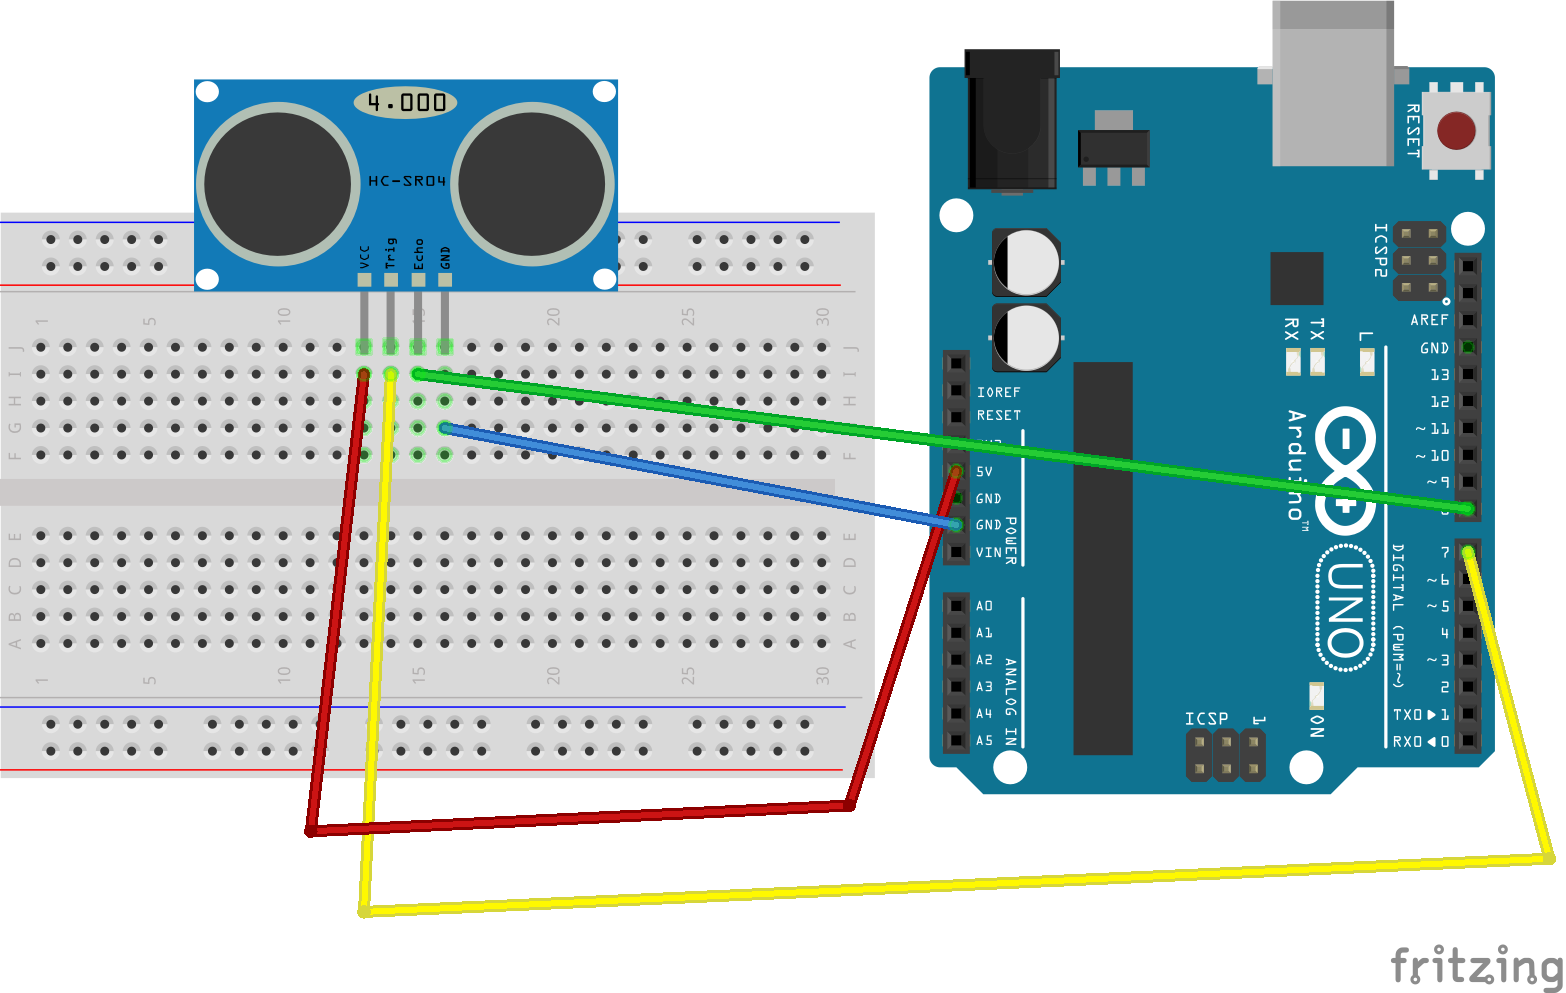
\includegraphics[width=7.0cm]{images/kadai7-1-1.png}
\caption{課題7.1.1のブレッドボード図}
\label{fig:kadai7-1-1}
\end{center}
\end{figure}

また,以下ソースコード\ref{code:kadai7-1-1}に実装したプログラムを示す.

\begin{lstlisting}[caption = 課題7.1.1,label=code:kadai7-1-1][H]
const int trig = 7; //Trigピンをデジタル7番に接続
const int echo = 8; //Echoピンをデジタル8番に接続
unsigned long interval; //Echoのパルス幅
unsigned long velocity; //音の速度
unsigned long distance; //対象までの距離
void setup() {
  Serial.begin(9600); //シリアルポートを9600kbpsに設定
  velocity = (0.61 * 25 + 331.5) *100; //音の速度(cm/s)を計算
  pinMode(trig,OUTPUT);
  pinMode(echo,INPUT);
}

void loop() {
  //10μsのパルスをTrigピンに出力
  digitalWrite(trig,HIGH);
  delayMicroseconds(10);
  digitalWrite(trig,LOW);

  //Echo信号がHIGHである時間(μs)をpulseIn関数で計測
  //5768μs以上経過したら,超音波が反射して帰ってこないとみなして0を返す
  //距離が100cm以上の時は0を返す
  //0.61 * 25 + 331.5 = 346.75
  //346.75 * x*100/2 = 100.0
  //x = 5768 
  interval = pulseIn(echo,HIGH,5768); 
  //
  distance = (velocity * interval / 1000000 ) / 2 ; //距離を計算(cm)
  //Serial.println(interval); //超音波の往復時間をシリアルモニタに表示
  Serial.println(distance); //距離をシリアルモニタに出力
  delay(60); //次のTrig信号の出力まで60ms待機
}
\end{lstlisting}

purseIn関数の第3引数を大きくすると長い距離を測定することができるようになるが,その分次の距離を測定するまでの時間が長くなってしまう欠点があると考えられる.

\section{レポート7.1.2}
課題7.1.2で実装したプログラムを報告せよ. \\
距離の測定において,ボーリングによる計測とタイマ割り込みによる計測は,どのような状況で使い分けるべきか考察せよ. \\


以下ソースコード\ref{code:kadai7-1-2}に実装したプログラムを示す.
\begin{lstlisting}[caption = 課題7.1.2,label=code:kadai7-1-2][H]
#include<MsTimer2.h>
const int trig = 7; //Trigピンをデジタル7番に接続
const int echo = 8; //Echoピンをデジタル8番に接続
unsigned long interval; //Echoのパルス幅
unsigned long velocity; //音の速度
unsigned long distance; //対象までの距離
void setup() {
  Serial.begin(9600); //シリアルポートを9600kbpsに設定
  velocity = (0.61 * 25 + 331.5) * 100; //音の速度(cm/s)を計算
  pinMode(trig,OUTPUT);
  pinMode(echo,INPUT);
  MsTimer2::set(100,measure); //タイマ割り込み間隔100ms
  MsTimer2::start(); //タイマ割り込み開始
}

void measure() {
  //10μsのパルスをTrigピンに出力
  digitalWrite(trig,HIGH);
  delayMicroseconds(10);
  digitalWrite(trig,LOW);

  //Echo信号がHIGHである時間(μs)をpulseIn関数で計測
  //距離が100cm以上の時は0を返す
  //0.61 * 25 + 331.5 = 346.75
  //346.75 * x*100/2 = 100.0
  //x = 5768 
  interval = pulseIn(echo,HIGH,5768); 
  distance = (velocity * interval / 1000000 ) / 2 ; //距離を計算(cm)
  //Serial.println(interval); //超音波の往復時間をシリアルモニタに表示
  Serial.println(distance); //距離をシリアルモニタに出力
}
void loop() {
}
\end{lstlisting}

ポーリング処理の場合,delayを入れるがその際なんの処理もできないので,何か処理をしながら距離を測定したい場合はタイマ割り込みを用いるのが適切だと考えられる.

\section{レポート7.1.3}
課題7.1.3で作成した折れ線グラフと同心円図を報告せよ. \\
正確な距離計測をするには,どのような点に注意すればよいか,実験結果から考察せよ. \\

以下図\ref{fig:kadai7-1-3-oresen}に折れ線グラフを示す.

\begin{figure}[H]
\begin{center}
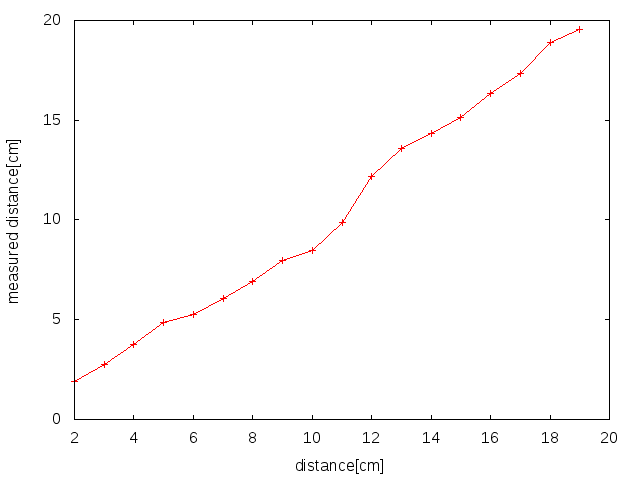
\includegraphics[width=7.0cm]{images/kadai7-1-3.png}
\caption{課題7.1.3の折れ線グラフ}
\label{fig:kadai7-1-3-oresen}
\end{center}
\end{figure}

また,以下図\ref{fig:kadai7-1-3-doushin}に同心円図を示す.

\begin{figure}[H]
\begin{center}
\includegraphics[width=7.0cm]{images/doushinenzu.JPG}
\caption{同心円図}
\label{fig:kadai7-1-3-doushin}
\end{center}
\end{figure}

図\ref{fig:kadai7-1-3-doushin}から,正確な距離測定をするにはある程度対象と超音波センサが正面で向かい合っているほうが良いと考えられる.また,測定対象も角度がついていると正確な距離測定ができないので,正面を向いている方がよいと考えられる.

\section{レポート7.1.4}
課題7.1.4で実装したブレッドボード図とプログラムを報告せよ. \\

以下図\ref{fig:kadai7-1-4}に実装したブレッドボード図を示す.

\begin{figure}[H]
\begin{center}
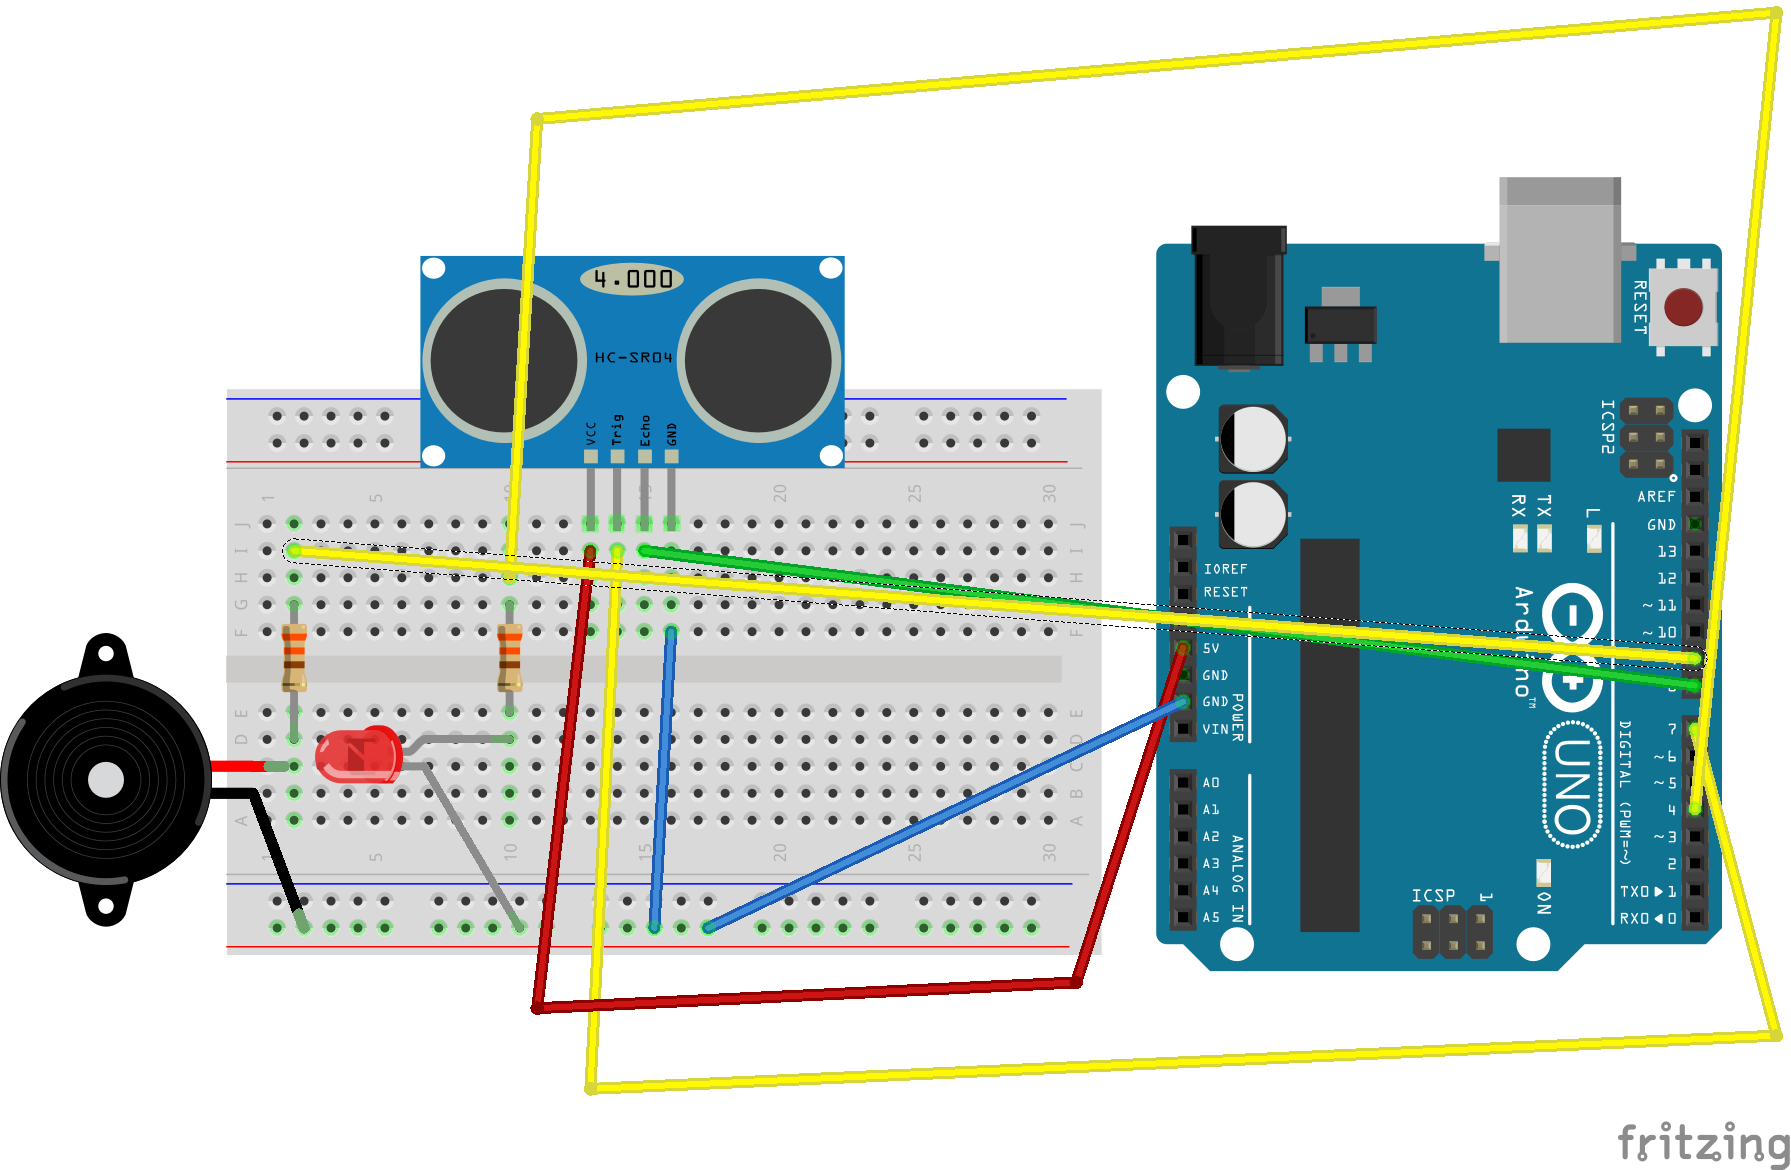
\includegraphics[width=7.0cm]{images/kadai7-1-4.png}
\caption{課題7.1.4のブレッドボード図}
\label{fig:kadai7-1-4}
\end{center}
\end{figure}

また,以下ソースコード\ref{code:kadai7-1-4}に実装したプログラムを示す.

\begin{lstlisting}[caption = 課題7.1.4,label=code:kadai7-1-4][H]
const int trig = 7; //Trigピンをデジタル7番に接続
const int echo = 8; //Echoピンをデジタル8番に接続
const int buzzer = 9; //圧電ブザーピンをデジタル9番に接続
const int led = 4; //ledピンをデジタル4番に接続
unsigned long interval; //Echoのパルス幅
unsigned long velocity; //音の速度
unsigned long distance; //対象までの距離
unsigned long frequency; //出力する周波数
void setup() {
  Serial.begin(9600); //シリアルポートを9600kbpsに設定
  velocity = (0.61 * 25 + 331.5) *100; //音の速度(cm/s)を計算
  pinMode(trig,OUTPUT);
  pinMode(echo,INPUT);
}

void loop() {
  //10μsのパルスをTrigピンに出力
  digitalWrite(trig,HIGH);
  delayMicroseconds(10);
  digitalWrite(trig,LOW);

  //Echo信号がHIGHである時間(μs)をpulseIn関数で計測
  //10000μs以上経過したら,超音波が反射して帰ってこないとみなして0を返す
  //距離が100cm以上の時は0を返す
  //0.61 * 25 + 331.5 = 346.75
  //346.75 * x*100/2 = 100.0
  //x = 5768 
  interval = pulseIn(echo,HIGH,10000); 
  //
  distance = (velocity * interval / 1000000 ) / 2 ; //距離を計算(cm)
  //Serial.println(interval); //超音波の往復時間をシリアルモニタに表示
  Serial.println(distance); //距離をシリアルモニタに出力
  if (distance <= 10) {
    digitalWrite(led,HIGH); //10cm以内ならled点灯
  }
  else {
    digitalWrite(led,LOW); //10cm以上ならled消灯
  }
  //距離が30を超えてたら30にする
  if( distance >= 30) distance = 30;
  //距離が0cmの時1000Hz,30cmの時100
  frequency = 1000 - (distance * 30); 
  tone (buzzer, frequency);
  delay(60); //次のTrig信号の出力まで60ms待機
}
\end{lstlisting}

\section{レポート7.1.5}
課題7.1.5で実装したブレッドボード図とプログラムを報告せよ. \\
サーボモータを指定した速度で開店させるために考慮した点を解説せよ. \\

以下図\ref{fig:kadai7-1-5}に実装したブレッドボード図を示す.

\begin{figure}[H]
\begin{center}
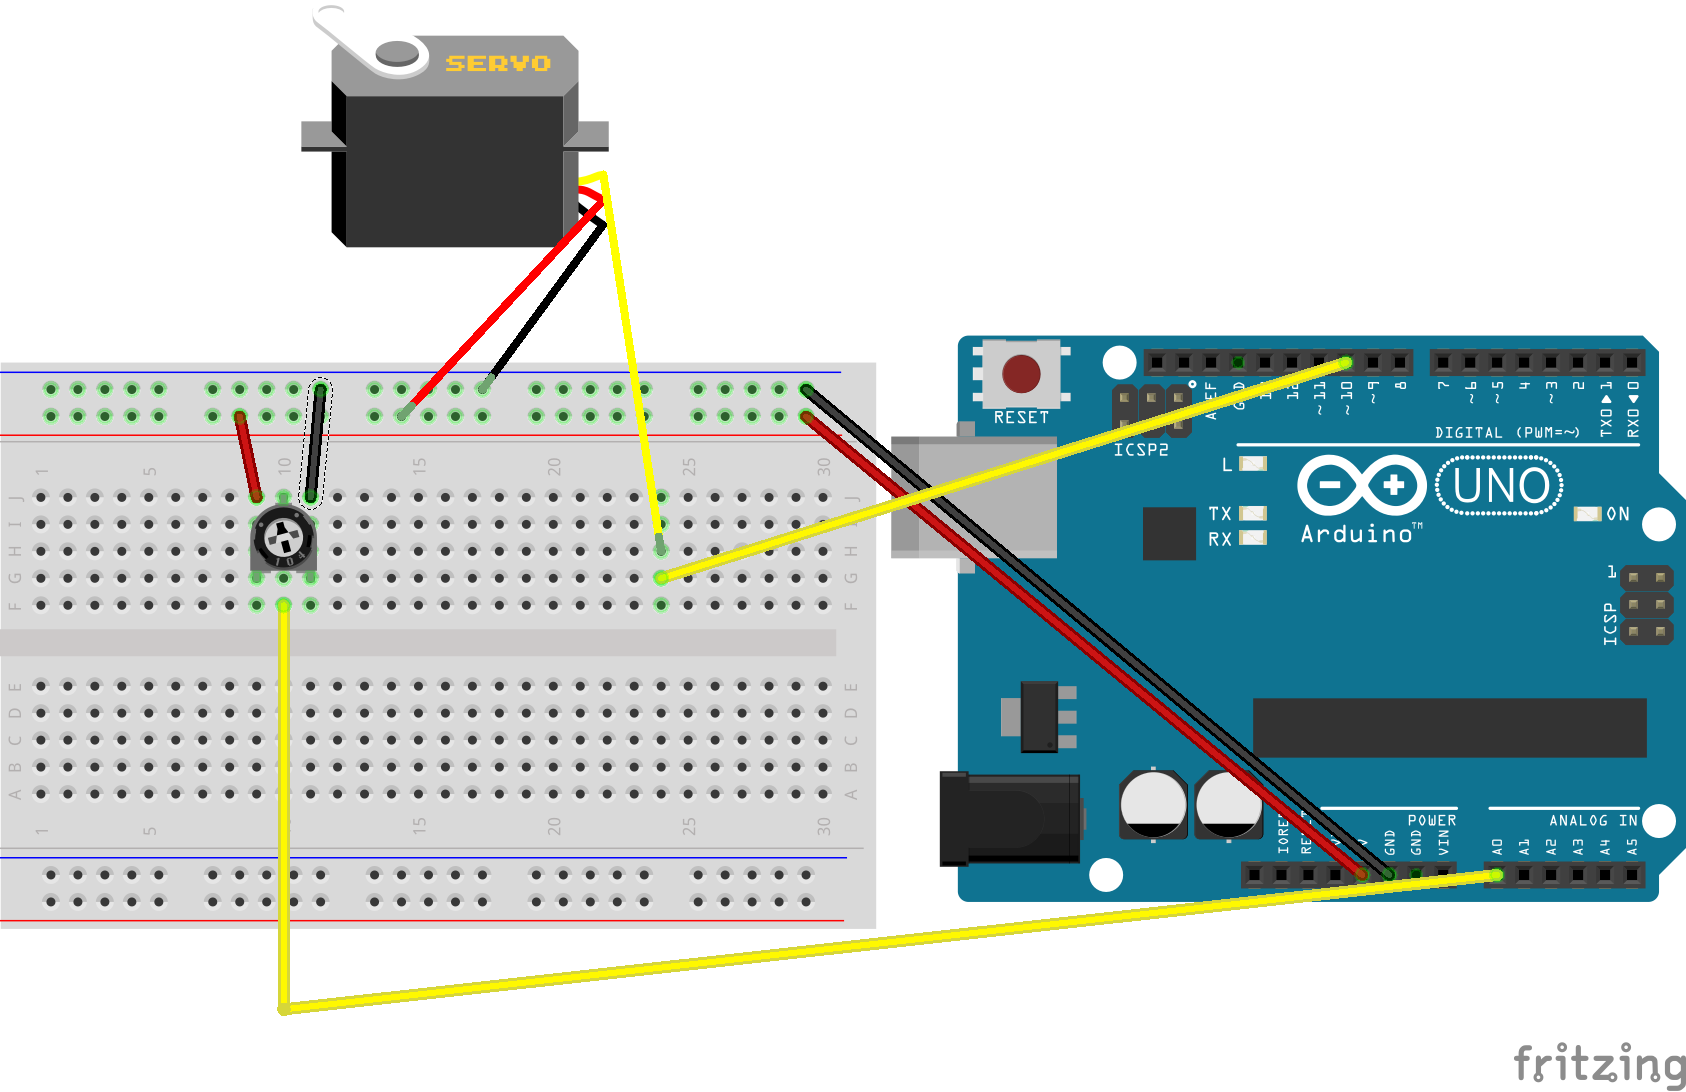
\includegraphics[width=7.0cm]{images/kadai7-1-5.png}
\caption{課題7.1.5のブレッドボード図}
\label{fig:kadai7-1-5}
\end{center}
\end{figure}


また,以下ソースコード\ref{code:kadai7-1-5}に実装したプログラムを示す.
\begin{lstlisting}[caption = 課題7.1.5,label=code:kadai7-1-5][H]
#include<Servo.h> //サーボライブラリのインクルード

Servo servo; //Servoクラスのインスタンスを生成

const int servoPin = 10; //サーボモータの信号線をデジタル10番ピンに接続
int angle; //回す角度
int sensorvalue; //半固定抵抗の値
float wait; //待機時間
boolean clockwise = false; //時計回りかどうか
void setup() {
 servo.attach(servoPin); //制御の対象を10番ピンに割当
 Serial.begin(9600);
 angle = 0;
}

void loop() { 
  sensorvalue = analogRead(A0); //A0ピンのAD変換結果を取得(半固定抵抗の値)
  servo.write(angle);
  if (clockwise)  angle--; //時計回りなら角度を小さくしていく
  else {
    angle++; //半時計回りなら角度を大きくしていく
  }
  if (angle == 180) clockwise = true; //角度が180に到達したら時計回りに変更
  if (angle == 0) clockwise = false; //角度が0に到達したら半時計回りにする
  Serial.println(angle);
  Serial.println(sensorvalue);
  /*
  戻ってくるまでの回転は合計360度
  5秒で360度回転するということは
  1度の回転にかかる時間は5/360秒
  msに直すと
  5000/360ms ≒14ms
  18秒も同様に考えて
  18/360秒
  msに直して
  50ms
  */
  wait = map(sensorvalue,0,1023,14,50);// 0~1023のセンサの値を14~50に変換
  Serial.println(wait); //確認用
  delay(wait); //待ち時間(1度回転あたりの秒)
}
\end{lstlisting}
サーボモータを指定した速度で回転させるためにmap関数を利用した.一度180度回転してからもう一度戻ってくるので回転する合計の角度は
\begin{equation}
180 \times 2 = 360
\end{equation}
で360度.5秒で1回転したい場合は1度にかかる時間をmsで書くと
\begin{equation}
\frac{5000}{360} \simeq 14ms
\end{equation}
18秒も同様に考えると
\begin{equation}
\frac{18000}{360} \simeq 50ms
\end{equation}
これから,map関数でセンサの値により14msから50msまで変えた.ソースコード\ref{code:kadai7-1-5}のコメントにもこれらを記述している.
\end{document}
